\author{@Teebor-Choka, @slobodaapl}
\documentclass[11pt,english,a4paper,openany]{book}
\usepackage[a4paper,top=3.5cm,bottom=3.5cm,left=3cm,right=3cm,marginparwidth=1.75cm]{geometry}
\newcommand{\myFontSize}[0] {12pt}
\usepackage[IL2]{fontenc}
\usepackage[utf8]{inputenc}
\usepackage{url}
\usepackage{ifthen}
\usepackage[hidelinks]{hyperref}
\usepackage{graphicx}
\usepackage{listings}
\usepackage{titlesec}
\usepackage{subcaption}
\usepackage{float}
\usepackage{amsmath}
\usepackage{amssymb}
\usepackage{amsfonts}
\usepackage{amstext}
\usepackage{amsthm}
\usepackage[style=iso-numeric,sorting=none]{biblatex}
\addbibresource{references.bib}
\usepackage{etoolbox}
\apptocmd{\sloppy}{\hbadness 10000\relax}{}{}
\newcommand{\myparagraph}[1]{\paragraph{#1}\mbox{}\vspace{8pt}\\}
\newcommand{\mysubparagraph}[1]{\paragraph*{#1}\mbox{}\vspace{8pt}\\}
\edef\restoreparindent{\parindent=\the\parindent\relax}
\usepackage{parskip}
\restoreparindent
\usepackage{enumitem}
\setlist[itemize]{parsep=3pt}
\setlist[enumerate]{parsep=3pt}
\addtolength{\topskip}{0pt plus 10pt}
\newcounter{parno}
\makeatletter
\renewcommand{\thesection}{\arabic{section}}
\newcommand{\newparb}[2]{\global\@namedef{mypar@b#1}{#2}}
\newcommand{\newpare}[2]{\global\@namedef{mypar@e#1}{#2}}
\newpare{0}{0}
\let\oldpar\par
\def\par{\oldpar\protected@write\@auxout{}{\string\newpare{\theparno}{\thepage}}}
\makeatother
\emergencystretch=1em
\usepackage[splitrule]{footmisc}
\interfootnotelinepenalty=10000
\widowpenalties 1 10000
\raggedbottom
\usepackage{listings}
\usepackage{color}
\usepackage{titling}
\renewcommand\maketitlehooka{\null\mbox{}\vfill}
\renewcommand\maketitlehookd{\vfill\null}
\usepackage{etoolbox}
\makeatletter
\providecommand{\subtitle}[1]{% add subtitle to \maketitle
\apptocmd{\@title}{\par {\large #1 \par}}{}{}
}
\makeatother
\usepackage{titlesec}
\setcounter{secnumdepth}{4}

\usepackage{color}
\usepackage{xcolor}
\colorlet{punct}{red!60!black}
\definecolor{background}{HTML}{EEEEEE}
\definecolor{delim}{RGB}{20,105,176}
\colorlet{numb}{magenta!60!black}

% language definitions
\lstdefinelanguage{json}{
    basicstyle=\normalfont\ttfamily,
    numbers=left,
    numberstyle=\scriptsize,
    stepnumber=1,
    numbersep=8pt,
    showstringspaces=false,
    breaklines=true,
    frame=lines,
    backgroundcolor=\color{background},
    literate=
     *{0}{{{\color{numb}0}}}{1}
      {1}{{{\color{numb}1}}}{1}
      {2}{{{\color{numb}2}}}{1}
      {3}{{{\color{numb}3}}}{1}
      {4}{{{\color{numb}4}}}{1}
      {5}{{{\color{numb}5}}}{1}
      {6}{{{\color{numb}6}}}{1}
      {7}{{{\color{numb}7}}}{1}
      {8}{{{\color{numb}8}}}{1}
      {9}{{{\color{numb}9}}}{1}
      {:}{{{\color{punct}{:}}}}{1}
      {,}{{{\color{punct}{,}}}}{1}
      {\{}{{{\color{delim}{\{}}}}{1}
      {\}}{{{\color{delim}{\}}}}}{1}
      {[}{{{\color{delim}{[}}}}{1}
      {]}{{{\color{delim}{]}}}}{1},
}
\definecolor{lightgray}{rgb}{.9,.9,.9}
\definecolor{darkgray}{rgb}{.4,.4,.4}
\definecolor{purple}{rgb}{0.65, 0.12, 0.82}
\lstdefinelanguage{JavaScript}{
  keywords={break, case, catch, continue, debugger, default, delete, do, else, false, finally, for, function, if, in, instanceof, new, null, return, switch, this, throw, true, try, typeof, var, void, while, with},
  morecomment=[l]{//},
  morecomment=[s]{/*}{*/},
  morestring=[b]',
  morestring=[b]",
  ndkeywords={class, export, boolean, throw, implements, import, this},
  keywordstyle=\color{blue}\bfseries,
  ndkeywordstyle=\color{darkgray}\bfseries,
  identifierstyle=\color{black},
  commentstyle=\color{purple}\ttfamily,
  stringstyle=\color{red}\ttfamily,
  sensitive=true
}

\lstset{
   language=JavaScript,
   backgroundcolor=\color{lightgray},
   extendedchars=true,
   basicstyle=\footnotesize\ttfamily,
   showstringspaces=false,
   showspaces=false,
%    numbers=left,
   numberstyle=\footnotesize,
   numbersep=9pt,
   tabsize=2,
   breaklines=true,
   showtabs=false,
   captionpos=b
}

\begin{document}
\title{EVA Gallery Design Document}
\subtitle{Digital Art Experience enhanced with AI and web3 (Milestone 2)}
\date{\today}
\maketitle

\thispagestyle{empty} % Ensures the title page has no page number

\newpage
\newgeometry{top=2.5cm,bottom=2.5cm,left=3cm,right=3cm}
\tableofcontents
\thispagestyle{empty}
\addtocontents{toc}{\protect\thispagestyle{empty}}
\restoregeometry

\pagestyle{plain}
\pagenumbering{arabic}

\chapter{Features}

\section{AI: Art Theft Protection}
Implementation of a multi-layered approach to safeguarding artists' work, including:

    \begin{itemize}
        \item \textbf{Nightshade:} A cutting-edge technique~\cite{shan2024nightshade} that subtly alters artwork to render it useless for AI training while maintaining visual fidelity for human viewers.
        \item \textbf{NFT Minting (Non-AI pre-existing):} Using blockchain technology to create NFTs for each artwork, ensuring verifiable authenticity and ownership.
        \item \textbf{Metadata Integration:} Leveraging standardized metadata formats to store essential information about the artwork, including artist attribution, ownership details, and licensing terms.
    \end{itemize}

\subsection{Protection from use in AI models}

Nightshade is a pioneering technique designed to protect artists' work from being exploited for training AI models. It introduces imperceptible perturbations to the image data, rendering it ineffective for AI training while preserving visual fidelity for human observers~\cite{shan2024nightshade}. This approach ensures that the artwork remains visually appealing and unaltered for human consumption, while effectively "poisoning" the data for AI algorithms.

\begin{figure}[ht]
    \centering
    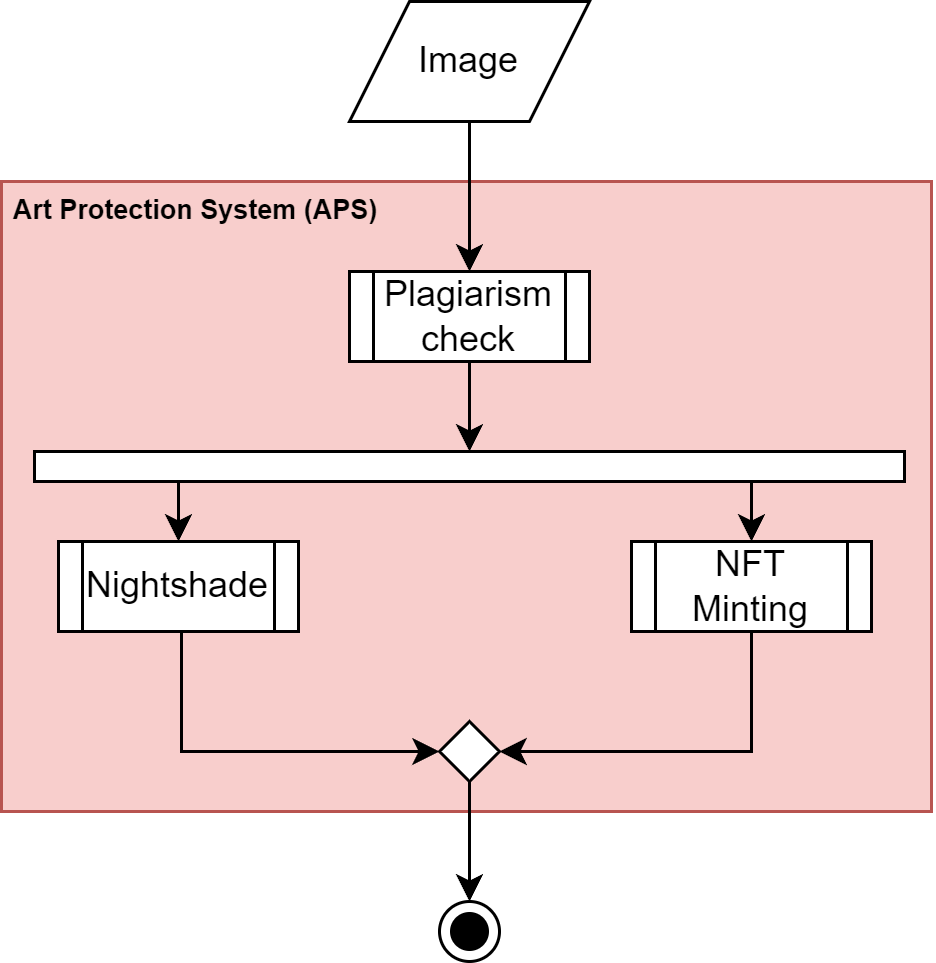
\includegraphics[width=0.8\textwidth]{figs/aps.png}
    \caption{Data flow through the processes for the Art Protection System in EVA Gallery.}
    \label{fig:data_flow}
\end{figure}

A similar tool, Glaze, focuses on protecting against style theft by subtly altering artwork to disrupt AI models' ability to mimic an artist's unique style~\cite{shan2023glaze}. However, Nightshade and Glaze are not yet interoperable, limiting their combined effectiveness in protecting against both content and style theft. EVA Gallery will monitor the development of these tools and integrate them when feasible to provide comprehensive protection against AI-powered art theft.

\subsection{Plagiarism check: a two-pronged approach}

EVA Gallery's plagiarism detection system employs a robust two-pronged approach to ensure the originality of uploaded artwork and protect artists' intellectual property rights, shown in~\autoref{fig:data_flow}.

\subsubsection{Embedding-based similarity check}

The first step involves converting the uploaded artwork into a high-dimensional numerical representation called an embedding. This embedding captures the semantic content of the image, including its objects, scenes, and overall meaning. The embedding is then compared against all existing embeddings in the database using efficient similarity search techniques like HNSW indexing. If an extremely close match is found, the artwork is flagged for further inspection.

\subsubsection{Gramian matrix similarity check}

Flagged images undergo a second level of scrutiny using Gramian matrix analysis. A Gramian matrix is a mathematical representation that captures the style of an image, including its textures, colors, and patterns. It is calculated from the feature maps extracted from the image by a pre-trained neural network.

Gramian matrices have been widely used in style transfer tasks, where the style of one image is transferred onto the content of another~\cite{nicolas2019improving}. However, their potential for style similarity comparison in the context of plagiarism detection is also promising. By comparing the Gramian matrix of the flagged image with those of existing artworks in the database, we can assess the degree of stylistic similarity. If a high match is found even at this stage, the artwork is flagged for human inspection.

This two-pronged approach provides a comprehensive check for plagiarism, considering both the semantic content and stylistic elements of the artwork. The embedding-based similarity check efficiently narrows down potential matches, while the Gramian matrix analysis delves deeper into the stylistic nuances to identify potential cases of plagiarism that may not be apparent from content alone.

By implementing this rigorous plagiarism detection system, EVA Gallery aims to create a fair and transparent platform where artists can showcase their work with confidence, knowing that their creations are protected from unauthorized copying and misuse.

\newpage
\section{AI: Plagiarism Protection}
Employ advanced techniques to detect and prevent plagiarism, ensuring the originality of uploaded artwork.

    \begin{itemize}
        \item \textbf{Embedding Space Lookup:} Artwork will be converted into numerical representations (embeddings) and compared within a vast database of existing art to identify potential copies or derivatives.
        \item \textbf{Gramian Matrix Similarity (Pending Research):}\footnote{Further research is needed to validate the effectiveness of this method for plagiarism detection.} A potential method that could further enhance plagiarism detection by analyzing the structural similarities between artworks.
        \item \textbf{Two-pronged Protection:} This system will guarantee that no modified artwork can be uploaded without proper attribution and permission, safeguarding artists' rights and fostering a fair creative environment.
    \end{itemize}

\newpage

\section{AI: Art Recommendation Engine}
Provide personalized recommendations to users based on their preferences and interactions with the artwork.

\begin{itemize}
    \item \textbf{Multi-Faceted Similarity:} Recommendations will consider both stylistic and content-based similarity to provide a diverse and engaging selection of artwork based on currently observed or displayed artwork.
    \item \textbf{Gramian-Based Style Recommendations:} Style-similar artwork will be evaluated using Gramian matrix similarity if proven viable.
    \item \textbf{Embedding-Based Content Recommendations:} Context-similar artwork will be displayed with respect to the typical similarity between embedded representations with MetaCLIP model.
    \item \textbf{Art Search:} Users will be able to input text that will be embedded and used to obtain images that most closely match the query.
\end{itemize}

\subsection{Embedding-based content recommendations}
EVA Gallery will take advantage of the power of image embeddings to provide content-based recommendations. By comparing the embedding of a user's observed artwork with the embeddings of other artworks in the database, we can identify pieces with similar semantic content, such as shared themes, subjects, or concepts. This enables us to recommend artworks that are similar to the currently observed artwork.

\subsection{Mixed recommendations (embeddings and Gramian matrices)}
To offer a diverse range of recommendations, we also consider a mixed approach that combines both embedding-based content similarity and Gramian matrix-based style similarity. This allows us to recommend artworks that share similar themes and visual styles with the observed artwork, providing a more comprehensive and engaging recommendation experience.

By incorporating both content and style information, we can cater to users who are interested in exploring artworks with similar subjects but different styles, or vice versa. This approach enhances the discovery aspect of the platform, exposing users to a wider array of artistic expressions.

\subsection{Gramian-based style recommendations}
For users who are primarily interested in visual styles, we offer recommendations based solely on Gramian matrix similarity. This allows us to identify artworks that share similar textures, colors, and patterns with the user's liked pieces, regardless of their semantic content.

This feature is particularly useful for users who are seeking inspiration for their own artistic creations or who are interested in exploring different artistic styles within a specific genre. By focusing on visual similarity, we can provide recommendations that corresponds best with the currently displayed artwork.

\newpage

\chapter{User Stories}
\chapter{Workflows}
\section{Data pipeline: Image upload and processing workflow}

Upon uploading an image to EVA Gallery, the system generates its embedding using the MetaCLIP model. This embedding captures the semantic content of the image and serves as the primary basis for content-based similarity search and recommendations.

The generated embedding is compared against all existing embeddings in the vector database using efficient similarity search techniques like HNSW indexing. If a close match is found, indicating potential plagiarism, the system extracts a Gramian matrix from either the encoded representation feature maps or from pre-computed matrices stored in the database. This Gramian matrix is then compared against the Gramian matrix of the uploaded image to assess the degree of stylistic similarity. If a high match is detected, the image is flagged for human review to determine whether it constitutes plagiarism. This and the whole pipeline is visualized in~\autoref{fig:pipeline}.

\begin{figure}[ht]
    \centering
    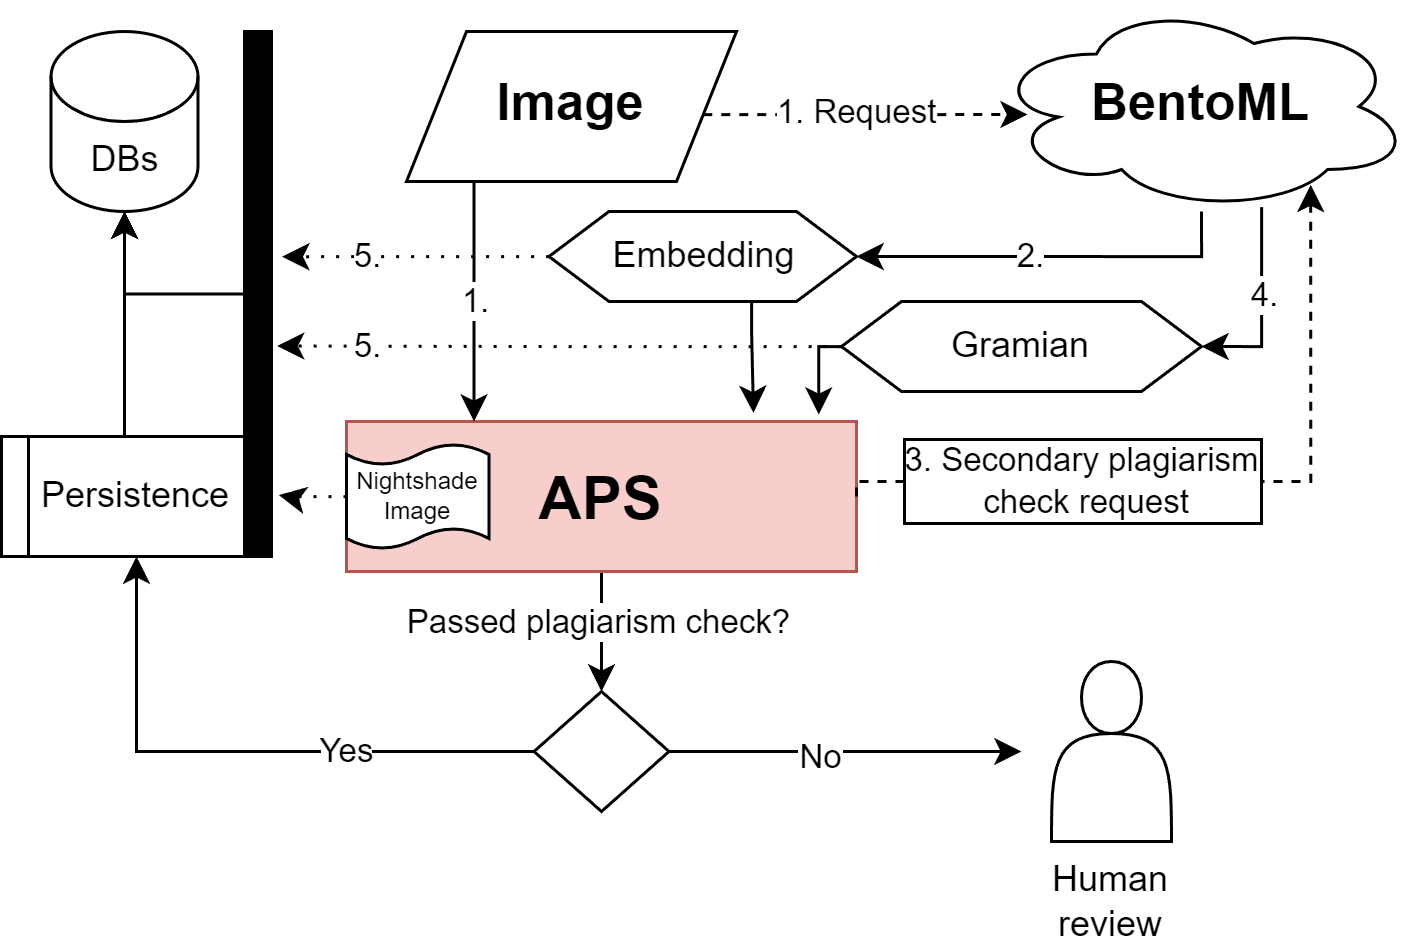
\includegraphics[width=0.8\textwidth]{figs/integ.png}
    \caption{Integration schema of the data pipeline, in other words, the image flow through the connected components of the system and the related infrastructure.}
    \label{fig:pipeline}
\end{figure}

Images that pass the plagiarism check are stored in the database along with their corresponding embeddings and Gramian matrices. Additionally, relevant metadata, including artist attribution, ownership details, and licensing terms, is associated with the image.

The artist has the option to mint the uploaded artwork as an NFT. The image is also processed with Nightshade, introducing subtle perturbations to render it useless for AI training while preserving visual fidelity. The Nightshade-processed image is stored as a separate copy in the database, linked to the original image via its unique UUID. This modified image is then displayed in the gallery, ensuring that visitors interact with the protected version while the original remains secure.

\newpage

\chapter{System Requirements}
\section{AI}
\begin{enumerate}
\item \textbf{Database Access:}
    \begin{itemize}
    \item Access to a database of existing images (UUID identified).
    \item Storage for modified images (Nightshade) alongside originals.
    \end{itemize}
\item \textbf{Vector Database:}
    \begin{itemize}
    \item Storage for embeddings and Gramian matrices.
    \item HNSW indexing for efficient similarity search.
    \end{itemize}

\item \textbf{Cloud Backend:}
    \begin{itemize}
    \item Hosts MetaCLIP (embeddings) and ResNet (Gramian matrices) models.
    \item Supports batched input.
    \item Simple API (e.g., BentoML).
    \end{itemize}

\item \textbf{Hardware Requirements:}
    \begin{itemize}
    \item MVP: GPU with at least 24GB VRAM.
    \item Deployment: Scalable GPU compute with load balancing and in-flight batching
    \end{itemize}
\end{enumerate}

\newpage

\chapter{Technology stack}
\section{AI}

\begin{enumerate}
\item \textbf{Database Access:}
    \begin{itemize}
        \item \textbf{PostgreSQL:} A robust open-source relational database management system, offering support for structured data, ACID compliance, and scalability. Ideal for storing image metadata and maintaining associations between original and modified images.
    \end{itemize}

\item \textbf{Vector Database:}
    \begin{itemize}
        \item \textbf{pgvector+pgvectorscale+cube:} A PostgreSQL extension adding support for vector data types with similarity search using indexing algorithms, and matrix storage and search with cube. Cost-effective and scalable for storing and searching embeddings and Gramian matrices.
    \end{itemize}

\item \textbf{Cloud Backend:}
    \begin{itemize}
        \item \textbf{BentoML:} A flexible framework for building and deploying machine learning services. Simplifies packaging and deployment of models, allowing easy integration with various cloud providers, and supports batched input processing and API generation.
        \item \textbf{Self-hosted:} Kubernetes provides control and flexibility in configuring the software environment and automating deployment and building. We can utilize our existing servers with a proper MLDevOps architecture to ensure CI and CD alongside AI models.
    \end{itemize}

\item \textbf{Scalable GPU Compute:}
    \begin{itemize}
        \item \textbf{Nvidia Triton Inference Server:} A high-performance inference server optimized for serving deep learning models. Supports dynamic batching and model ensemble, maximizing GPU utilization and throughput. Integrates with Kubernetes for seamless scaling and management.
    \end{itemize}
\end{enumerate}

\newpage

\begingroup
    \hbadness 10000
    \relax
    \printbibliography
\endgroup

\end{document}
